\documentclass{template/openetcs_article}
%\documentclass{article}
%\usepackage[ascii]{inputenc}
%\usepackage[T1]{fontenc}
\usepackage[english]{babel}
\usepackage{amsmath}
\usepackage{amssymb,amsfonts,textcomp}
\usepackage{array}
\usepackage{supertabular}
\usepackage{hhline}
\usepackage{graphicx}
\makeatletter
\newcommand\arraybslash{\let\\\@arraycr}
\makeatother
\setlength\tabcolsep{1mm}
\renewcommand\arraystretch{1.3}
\newcounter{Ilustracin}
\renewcommand\theIlustracin{\arabic{Ilustracin}}
\title{openETCS}

%\setcounter{tocdepth}{3}
\usepackage{float}
\usepackage{hhline}
\usepackage{booktabs}
\usepackage{multirow}
\usepackage{color, colortbl}
\definecolor{myblue}{rgb}{0.6,.6,1}
\definecolor{mydarkblue}{rgb}{0,0,0.5}
\definecolor{mylightblue}{rgb}{0.8,0.8,1}
\usepackage{hyperref}
\hypersetup{colorlinks=true, linkcolor=mydarkblue, urlcolor=mydarkblue}

\usepackage[textwidth=2.7cm,textsize=scriptsize,linecolor=green!40,backgroundcolor=green!40]{todonotes}

\newcounter{mycommentcounter}
\newcommand{\mycomment}[2][]
{
\refstepcounter{mycommentcounter}%
\todo[color={red!100!green!33}]{
\textbf{[\uppercase{#1} \themycommentcounter]:} #2}
}


\usepackage{lipsum,url}
\graphicspath{{./template/}{.}{./images/}}
\begin{document}
\frontmatter
\project{openETCS}

%Please do not change anything above this line
%============================
% The document metadata is defined below

%assign a report number here
\reportnum{OETCS/WP1/D1.3.1}

%define your workpackage here
\wp{Work-Package 1: ``Management''}

%set a title here
\title{Project Quality Assurance Plan - Revision Process}

%set a subtitle here
%\subtitle{A template for short document. Adapted from report template.}

%set the date of the report here
\date{\today}

%define a list of authors and their affiliation here

\author{SQS}

\affiliation{Avda. Zugazarte 8,6\\
  48930 Getxo \\
  Vizcaya, España}


% define the coverart
\coverart[width=350pt]{openETCS_EUPL}

%define the type of report
\reporttype{Description of work}




%=============================
%Do not change the next three lines
\maketitle
\tableofcontents
%\listoffiguresandtables
\newpage
%=============================

% The actual document starts below this line
%=============================


%Start here



%\begin{document}


\section*{Document History}

\begin{flushleft}
%\tablefirsthead{\hline Version & Date & Chapters modified & Reason & Name\\}

\tablehead{\hline \rowcolor{myblue} Version & Date & Chapters modified & Reason & Name\\}

\tabletail{}
\tablelasttail{}
\begin{supertabular}{m{1.1cm}m{1.8cm}m{2cm}m{7cm}m{2cm}lp{6cm}|}
\hline
0.0.1 &
09.04.2013 &
All &
First version &
SQS
\\\hline
0.0.2 &
12.04.2013 &
Roles &
Tables added to the 'Roles' section &
SQS
\\\hline
0.0.3 &
15.04.2013 &
T.instructions &
Technical instructions completed &
SQS
\\\hline
0.0.4 &
16.05.2013 &
All &
Comments of the reviewers analysed and some changes implemented &
SQS
\\\hline
0.0.5 &
23.05.2013 &
All &
New complete version adjusted to the Revision process concept &
SQS
\\\hline
0.0.6 &
06.06.2013 &
All &
New complete version adjusted to the Revision process concept &
SQS
\end{supertabular}
\end{flushleft}

\newpage

\section{Introduction}

\subsection[Introduction]{Purpose of the document}
This document presents the whole process to follow when documents need revision. It aims to provide a set of guidelines as technical instructions for each revision cycle launched that highlights the steps to take.The roles involved in the process are clearly identified as well as their responsibilities and tasks. And finally, the mechanisms needed to achieve the proposed objectives are also included, so the process can be carried out successfully.

\subsection{Intended Audience}
This document applies to the whole development life-cycle of the project and it addresses all the Author(s), Committers and Contributors involved. This document should be available to all of them in read access mode and it provides guidance about the Revision process to follow anytime revisions of documents are needed.

\subsection{Supporting documents}
\tablefirsthead{\hline
\rowcolor{myblue}
Name &
Path &
Contents\\}
\tablehead{}
\tabletail{}
\tablelasttail{}
\begin{supertabular}{|m{2cm}m{3cm}m{9cm}|}
\hline
Todonotes package &
governance/Review Process &
Brief introduction to the todonotes package with detailed descriptions about the available attributes. 
\\\hline
Revision Guidelines &
Governance/Review Process &
It describes major aspects to be assessed during a Revision Cycle.
\\\hline
QA Plan &
Governance/QA Plan &
It defines the processes, methods and tools that will be used to develop the OpenETCS project.
\\\hline
\end{supertabular}

\subsection{Definitions and acronyms}
\tablefirsthead{\hline
\rowcolor{myblue}
Abbreviation &
Meaning\\}
\tablehead{}
\tabletail{}
\tablelasttail{}
\begin{supertabular}{|m{3cm}m{11cm}|}
\hline
Revision Process &
It is the process through which committers and selected contributors perform a through analysis of a document, propose contributions and improvements to be included before the document is published in the OpenETCS repository.
\\\hline
Review Process &
It is the process through which the OpenETCS community is invited to make comments and suggestions, propose corrections and improvements to a document.
\\\hline
RC &
Revision Cycle.
\\\hline
Committer &
A person who has editing rights for a specific project.
\\\hline
Contributor &
A person without editing rights for a project that contributes with comments or improvements. A Contributor can become a Committer through a voting process.
\\\hline  
\end{supertabular}

\section{Tools}

\begin{flushleft}

\begin{tabular}{|m{3cm}|m{11cm}|}
\hline
\rowcolor{myblue}
\multicolumn{2}{|c|}{Tools} \\\hline
GIT &
\begin{itemize}
\item GitHub: A web-based hosting service for projects that use Git revision control system.
\item SmartGit: A graphical front-end for Git distributed version control systems. 
\end{itemize}\\\hline
Pdf documents &
\begin{itemize}
\item Adobe Acrobat Reader: Software package that allows to view, navigate and print pdf files.
\item Diffpdf: Open source application that compares different PDF files for discrepancies. 
\item {PDF Creator: Software for creating pdf files. Works like a printer on your PC.}
\end{itemize}\\\hline
TeX documents &
\begin{itemize}
\item MiKTeX : Provides the tools necessary to prepare documents using de TeX/LaTeX mark up language.
\item GhostScript. 
\item GhostView.
\item TexMaker.
\item Todonotes package.
\item Adobe Acrobat Reader: Software package that allows to view, navigate and print pdf files.
\end{itemize}\\\hline
\end{tabular}
\end{flushleft}

\section{Revision Process overview}

The revision process will be performed:
\begin{itemize}
\item After a first version of the document is created by the authors and when it is plausible significant contributions are still needed to have a complete and publishable document.
\item After a major rework of a document or after a review process in which major improvements/comments have been detected.
\end{itemize}
In all cases:
\begin{itemize}
\item The revision process will be carried out in a dedicated Revision Cycle Branch.
\item In case of conflicts, it is the Product Owner who will be responsible for their resolution
\item The Revision Team is composed of Committers and invited Contributors
\item Contributions/comments are made directly in the document under revision. However, in the case of “Contributors”, the Issue Tracker Tool will be used.
\item The launching, control and clarification processes are managed through the Issue Tracker Tool
\end{itemize}

\subsection{Structure of the repository}
 
The Revision process involves the creation of the following directory inside the structure of each repository once a {\it new branch} for the revision has been created.

\begin{flushleft}
\begin{tabular}{|m{3cm}|m{11cm}|}
\hline
\rowcolor{myblue}
\multicolumn{2}{|c|}{Structure of the repository} \\\hline
\rowcolor{lightgray}
Name &
Content 
\\\hline
Revision Documents &
\begin{itemize}
\item The document under revision: In Tex and PDF formats with all its history of changes, comments and sections added.
\end{itemize}\\\hline
\end{tabular}
\end{flushleft}

\subsection{Revision Roles}

This section describes the roles of the participants in the revision process of a document:

\begin{flushleft}
\begin{tabular}{|m{3cm}|m{11cm}|}
\hline
\rowcolor{myblue}
\multicolumn{2}{|c|}{Roles} \\\hline
\rowcolor{lightgray}
Role &
Competencies 
\\\hline
Product owner &
He/She is the main responsible of a document. 
He/She is in charge of launching the revision process; preparing the revision plan and controlling and monitoring the process progresses according to the plan; informing and interacting with the revision team members; approving and rejecting changes and resolving conflicts.
\\\hline
Author(s) & 
They provide support to the Product Owner in the revision of the contributions made by the revision team and therefore in the implementation of the approved ones. When requested by the Product Owner, they will provide support in assessing whether the document is ready for publication or not.
\\\hline
Revision Team &
As experts in the theme of the project, they will provide meaningful contributions to guarantee the document meets its scope and purpose  in a complete and accurate way.
\\\hline
\end{tabular}
\end{flushleft}

\subsection{Description of the Revision Process}

The next figure shows the different stages of the Revision Process. Right after the activities to be performed in each Stage are provided. The technical instructions on how to accomplish such activities are included in the Annex.

\begin{figure}[H]
\centering
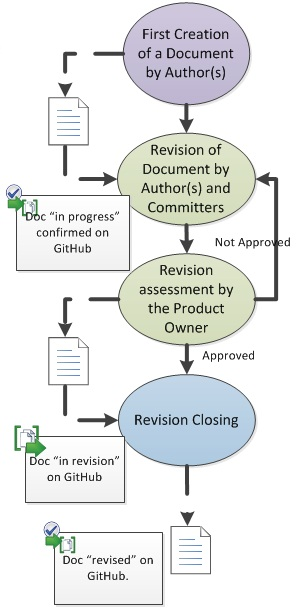
\includegraphics{./figures/RevisionProcess.JPG}
\caption{Revision Process flow}
\end{figure}

\subsubsection{Stage One: Launching of the Revision Process}

\begin{itemize}
\item The Product Owner elaborates a Revision Plan for the document with the envisaged deadlines for the different stages of the process and with the scope of the revision process itself. This information will be notified to the revision team members with the invitation.
\item The Product Owner creates the Revision Cycle Branch (RC Branch) and uploads the document to be revised to the RC Branch. Refer to {\it A1.Create a New RC Branch} in Annex for Technical Instructions.
\item The Product Owner updates the status of the document under revision in the wiki page “List of Documents” of the project to “In Revision”. Besides, a specific reference to the revision process is to be included in the ReadMe file.  
\item The Product Owner selects the revision team. 
\begin{itemize}
\item At least the Committers of the project where the project belongs to will be selected.
\item Contributors may also be invited to participate when considered appropriate.
\end{itemize}
\item The Product Owner invites the Committers and Contributors to participate. Refer to {\it A2.Revision Process-Control and Monitoring} in Annex for Technical Instructions.
\item The revision process starts officially.
\end{itemize}

\subsubsection{Stage Two: Revision process}
\begin{itemize}
\item Committers will be allowed to include the comments/contributions directly on the document under revision. Refer to {\it A3. Revision Activities} in Annex for technical instructions.
\item Once a committer finalizes with the revision, a notification will be sent to the Product Owner. Refer to {\it A3.Revision Activities} in Annex for Technical Instructions.
\item Contributors will make their comments/contributions as “Issues”. Refer to {\it A3. Revision Activities} in Annex for technical instructions.
\item The Product Owner with the support of the rest of the Author(s) of the document will analyze the comments/contributions as they arrive and when needed, interact with the appropriate revision team members asking for clarification. Refer to {\it A2.Revision Process-Control and Monitoring} in Annex for Technical Instructions.
\item The deadline for receiving comments may be extended by the Product Owner. Both the finalization and the extension will be notified to the revision team members. Refer to {\it A2.Revision Process-Control and Monitoring} in Annex for Technical Instructions.
\end{itemize}

\subsubsection{Stage Three: Approval Process}
\begin{itemize}
\item The Product Owner, with the support of the Authors, will approve and/or reject comments for final implementation. Refer to {\it A4. Approval/Rejection of Changes} for Technical Instructions.
\item Resolution of conflicts will be under the responsibility of the Product Owner
\item The Product Owner will implement the final changes in the document. Refer to section {\it A5. Final Implementation} for Technical Instructions.
\item The Product Owner will assess the comments received and will decide whether the document is ready for publication or not.
\item If it is not ready for publication, the Revision Cycle is re-opened by extending the deadline for receiving comments/contributions. Refer to {\it A2.Revision Process-Control and Monitoring} in Annex for Technical Instructions.
\item If the document is ready for publication, the Revision is ready to be closed. Refer to section {\it A6.Revision Closing} for technical instructions.
\end{itemize}


\subsubsection{Stage Four: Revision Closing}
\begin{itemize}
\item The Product Owner merges the RC Branch to the Master Branch. Refer to {\it A7.RC Branch Merging} in Annex for Technical Instructions.
\item The Product Owner updates the status of the document in the wiki to “Revised”. 
\item The Product Owner opens a “Review Process” for the document.
\end{itemize}

\section{ANNEXES - Technical Instructions}


\textbf{A1. Create a New RC branch}
\begin{flushleft}
\tablefirsthead{}
\tablehead{}
\tabletail{}
\tablelasttail{}
\begin{supertabular}{|m{2cm}|m{13cm}|}
\hline
\rowcolor{myblue}
TI & 
Create a New RC branch
\\\hline
Roles &
Product owner
\\\hline
Description &
Any changes made to the document to be revised shall be made in a RC branch context. The Product owner shall create the branch and makes it available for the revision team.
\\\hline
Steps &
\begin{itemize}
\item Steps to create the branch locally are:
\begin{enumerate}
   \item Open Smartgit
   \item Branch menu, add branch and give a new name following this nomenclature: 
   \begin{itemize}
   \item {\it RC\_<name of the document to be revised>\_<number of Revision>}. 
   \end{itemize}
   \item Push {\it add branch \& switch}. With these steps the branch is created as a local branch.
\end{enumerate}
\item Integrate the branch into the GitHub repository
\begin{enumerate}
	\item Go to the toolbar and press {\it Push}, accept then the messages. 
	\item The new branch appears in the Smartgit Branches view, below the origin tag. 
	\item Confirm that the local branch is linked to the remote GitHub branch: in the local branch the {\it set tracked branch shall} has been done and it shall address to the RC branch already created in the GitHub repository.
\end{enumerate}
\end{itemize}
\\\hline
\end{supertabular}
\end{flushleft}


\begin{figure}[H]
\centering
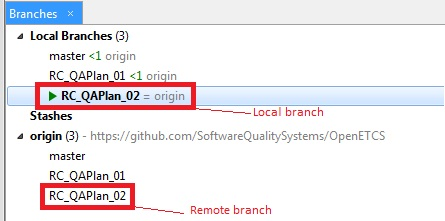
\includegraphics {./figures/Branches.JPG}
\caption{Branches tree in {\it Smartgit}}
\end{figure}

\textbf{A2. Revision Process-Control and Monitoring}

\begin{flushleft}
\tablefirsthead{}
\tablehead{}
\tabletail{}
\tablelasttail{}
\begin{supertabular}{|m{3cm}|m{12cm}|}
\hline
\rowcolor{myblue}
TI & 
Revision Process-Control and Monitoring
\\\hline
\rowcolor{lightgray}
Action &
Role/Instruction
\\\hline
Invitation to Participate to the Revision Team and launching the revision process &
Product Owner

Create a new Issue (Main Issue of the RC) in the Repository indicating a new RC is launched:
\begin{itemize}
\item Open Github and go to the correspondent repository
\item Select the {\it Issues section}
\item Push the {\it New issue} button
\item Add a descriptive title indicating the name of the new RC and the document under revision
\item Add a significant description about the causes that have motivated the new RC and summarizes the objectives of the revision. Provide the list of required Committers/Contributors.
\item Push {\it Submit new issue} 
\end{itemize}
If considered of interest, an e-mail can be sent to the invited people to the revision process
\\\hline
Interaction with the Revision Team to clarify comments &
Product Owner

Create an Issue addressing the corresponding Revision Team Member:
\begin{itemize}
\item Add a Title identifying the RC process
\item Add Text describing the details of the clarification requested
\end{itemize}
This Issue will be the Main Issue for the interaction with the expert. The rest of the communication will adopt the form of Comments to this Main Issue
\\\hline
Notification of Extension of the Revision Stage &
Product Owner

Add a Comment to the Main Issue of the RC indicating the deadline for receiving comments has been extended. The new deadline will be indicated.
\\\hline
Notification that the Revision Stage has finalized &
Product Owner

Add a Comment to the Main Issue of the RC indicating the date for receiving comments has finalized.
\\\hline
Notification the Revision Period has been re-opened &
Product Owner


Add a Comment to the Main Issue of the RC indicating the Revision period has been re-open and therefore a new deadline for receiving comments is indicated.

Besides specific indications for the process will be indicated.
\\\hline
\end{supertabular}
\end{flushleft}

\textbf{A3. Revision Activities}

\begin{flushleft}
\tablefirsthead{}
\tablehead{}
\tabletail{}
\tablelasttail{}
\begin{supertabular}{|m{2cm}|m{13cm}|}
\hline
\rowcolor{myblue}
TI & 
Revision environment setup
\\\hline
Roles &
Revision Team
\\\hline
Description &
Each Committer shall prepare the working environment locally and ensure it is ready before starting with the Revision tasks. The environment setup shall be optional for Contributors due to the do not have editing rights and they can have access to the documents to be downloaded directly from the GitHub website; in any case, they can configure the environment to have the documents locally, although they cannot edit them and {\it push} changes into the repository.
\\\hline
Steps &
\begin{itemize}
\item Setup using {\it Smartgit} tool
\begin{enumerate}
\item Clone the repository with the {\it Project --> Clone} option.
\item Go to the {\it Branch} menu, select {\it Add branch} and give a name. Then, the branch is created as a local branch.
\item Link the local branch to the remote git branch, to do that, select {\it Set tracked branch} in the context menu of the local branch. The local environment is then ready for working in the Revision Process
\end{enumerate}
\item Update the environment
\begin{itemize}
\item It is essential to work in the last version of the document under Revision, so minimal conflicts appear in the future when uploading the changes. To be sure about this, a pull request shall be done to the repository before editing the document.
\begin{itemize}
\item Select the {\it Pull} option on the toolbar
\end{itemize}
\end{itemize}
\end{itemize}
\\\hline
\end{supertabular}
\end{flushleft}

\begin{flushleft}
\tablefirsthead{}
\tablehead{}
\tabletail{}
\tablelasttail{}
\begin{supertabular}{|m{2cm}|m{13cm}|}
\hline
\rowcolor{myblue}
TI & 
Revision work
\\\hline
Roles &
Revision Team
\\\hline
Description &
The Committers and Contributors shall perform the revision in the expected time and conditions. The work of a Committer/Contributor shall finish when the Product owner confirms the closing of the RC.
\\\hline
Steps &
\begin{itemize}
\item The Committer shall:
\begin{enumerate}
\item Make comments, suggestions or improvement proposals with the {\it todonotes} (See {\it A10 Add notes using todonotes}).
\item Add comments in the RC issue thread when it applies (See {\it A11 Add comments in a RC issue}).
\item Make changes in the document. Each insertion shall be highlighted indicating the initials of the person involved. The Revision process shall be done by different people and what comments have been written by whom shall be known.
\end{enumerate}
\item The Committer shall integrate the changes into the document that is hosted in the remote repository in GitHub. To do that, click on the {\it Push} button in the SmartGit tool. When pushing different situations can happen:
\begin{itemize}
\item There are no conflicts with the original repository .
\begin{enumerate}
\item The changes shall be included.
\end{enumerate}
\end{itemize}
\begin{itemize}
\item There are one or more conflicts.
\begin{enumerate}
\item Click on the {\it Pull} button so the last version is loaded. 
\item Open the {\it Conflict Solver} Window to compare the committed version in the {\it Github} and the local version. 
\item The conflict shall be solved in the following way.
\begin{enumerate}
\item The Committer shall indicate that the version stored in the remote repository is the correct one. The changes in case of conflict are not included. 
\item The Committer will {\it Commit} and {\it Push} the changes that do not have any conflict and add a notification in the document about that. 
\item After finishing the {\it pushing}, he/she shall perform a {\it pulling} to obtain the integrated and last committed version; then he/she shall add a note using {\it todonotes} tool in the section where the conflicts were; he/she shall explain the problem found. 
\end{enumerate}
\item Have in mind that after {\it pushing/pulling} the document, the changes in conflict made by the Committer shall be lost. Anytime a conflict appears, the Committer shall prepare a copy of the suggestions or modifications made by him/her.
\item He/she also adds a comment in the RC issue thread (if it exists) or send an e-mail exposing that problem and requesting a solution.
\item The Author(s) and(or the Product owner shall take part in the discussion and propose a solution. The Committer can put in the document again the suggestions in conflict stored locally if the Author(s) or the Product owner requires that.
\end{enumerate}
\end{itemize}
\end{itemize}
\\\\\hline
Steps &
\begin{itemize}
\item The Contributor shall:
\begin{enumerate}
\item Make comments, suggestions or improvement proposals with the {\it Issue Tracker tool}.
\item Add comments in the RC issue thread when it applies (See {\it A11 Add comments in a RC issue}).
\end{enumerate}
\end{itemize}
\\\hline
Steps &
\begin{itemize}
\item In any case, the Committer/Contributor shall inform about the progress of the work posting a message in the RC issue thread or sending an e-mail. (See {\it A11 Add comments in a RC issue}).
\end{itemize}
\\\hline
\end{supertabular}
\end{flushleft}


\textbf{A4. Approval/Rejection of Changes}

\begin{flushleft}
\tablefirsthead{}
\tablehead{}
\tabletail{}
\tablelasttail{}
\begin{supertabular}{|m{2cm}|m{13cm}|}
\hline
\rowcolor{myblue}
TI & 
Approval/rejection of Changes
\\\hline
Roles &
Author(s)
\\\hline
Description &
The Author(s) shall study each proposal, recommendation or comment that appears in the document under revision and decide how to implement the proposed changes in case he/she estimates it is appropriate to be included in the document. On the other hand, and considering the Committers could include text in the document, the Author(s) shall assess the appropriateness of those sections and decide if this new content is accurate and relevant. When the contributions come from Contributors their issues shall be assessed due to they do not have editing rights.
\\\hline
Steps &
\begin{itemize}
\item When a Committer notifies that some changes have been pushed to GiThub using the corresponding RC branch, the Author(s) synchronizes their repository to obtain the last commit made for the document with the {\it SmartGit} tool.
\item The Author(s) reads carefully any annotation that appears in the document and decides whether the comments shall be implemented or not.
\item For each annotation the Author(s) find(s) in the document, a written confirmation about what is the decision about the subject shall be provided. 
\begin{enumerate}
\item Use the {\it todonotes} to confirm/reject proposals made by the Committers ({\it A10 Add notes using todonotes}) or to accept/delete new sections, text or paragraphs added by the Committers.
\item In any case, a justification for that decision shall be included.
\item When a suggestion is accepted:
\begin{enumerate}
\item Assess whether the recommendation made implies writing new paragraphs, sections, adding new figures, etc. and modify the document accordingly. 
\item Highlight the new text or the modified text with {\it todonotes} using the {\it inline} option.
\end{enumerate}
\end{enumerate}
\item Whenever a Contributor has added comments to an opened issue or has created a new one with contributions using the {\it Issue Tracker} tool, the Author(s) shall collect all the contributions reported, and assess the implementation of changes. The process shall be the same as in case of Committers but the tool to be in contact with the Contributor shall be the {\it Issue Tracker}.
\item The Author(s)commits the changes made in the document and push them into the RC branch so the Committers/Contributors can have access to the changes, confirmations and rejections made by the Author(s).
\item The Author(s) add(s) a message to the RC issue thread (if it exists) or send(s) an e-mail, so everyone can be informed about the commit recently done. 
\end{itemize}
\\\hline
\end{supertabular}
\end{flushleft}


\textbf{A5. Final Implementation}

\begin{flushleft}
\tablefirsthead{}
\tablehead{}
\tabletail{}
\tablelasttail{}
\begin{supertabular}{|m{2cm}|m{13cm}|}
\hline
\rowcolor{myblue}
TI & 
Final Implementation
\\\hline
Roles &
Product owner
\\\hline
Description &
The Product owner shall provide a final version with the considered changes implemented.  
\\\hline
Steps &
\begin{itemize}
\item Once the {\it Approval/rejection of comments} have been done, the changes implemented and pushed into the corresponding directory, a complete version of the document with those changes but without the comments shall be prepared.
\item The pdf and the original document shall be {\it commited} and {\it pushed} in the {\it Review Documents} directory.
\item A notification shall be included in the issue linked to the ongoing RC (if it exists) or send by e-mail: 
\begin{enumerate}
\item There, the Product owner shall explain that the changes have been implemented and that there is a complete version available in the corresponding path.
\end{enumerate}
\end{itemize}
\\\hline
\end{supertabular}
\end{flushleft}

\textbf{A6. Revision closing}

\begin{flushleft}
\tablefirsthead{}
\tablehead{}
\tabletail{}
\tablelasttail{}
\begin{supertabular}{|m{2cm}|m{13cm}|}
\hline
\rowcolor{myblue}
TI & 
Revision closing
\\\hline
Roles &
Product owner
\\\hline
Description &
The Product owner shall be the responsible for closing the current Revision Cycle after verifying and confirming all the changes done. The first task to be done is to notify the closing and highlight the results obtained.
\\\hline
Steps &
\begin{itemize}
\item Add a Comment in the Revision issue thread (if it exists) to indicate that the RC has finished
\begin{enumerate}
\item Follow the indications provided in the {\it A11 Add comments in a RC issue} to add a comment
\item Provide a brief summary of the RC:
\begin{enumerate}
\item Indicate the way the objectives have been met 
\item Are there pending objectives?. Indicate the reason for closing the RC before all the objectives have been met.
\item Identify the key aspects of the Revision
\item Highlight the results obtained
\end{enumerate}
\end{enumerate}
\item Close the RC issue thread pushing the {\it Close} button in {\it GitHub} when there is a Revision thread.
\item Or notify the closing of the RC sending an e-mail. The information included in this case is the same as before.
\end{itemize}
\\\hline
\end{supertabular}
\end{flushleft}

\textbf{A7. RC Branch merging}

\begin{flushleft}
\tablefirsthead{}
\tablehead{}
\tabletail{}
\tablelasttail{}
\begin{supertabular}{|m{2cm}|m{13cm}|}
\hline
\rowcolor{myblue}
TI & 
RC Branch merging
\\\hline
Roles &
Product owner
\\\hline
Description &
Merging the {\it RC Branch} to the {\it Master branch} implies incorporating the changes made in a document to the main branch of the repository. In this way, the new version of the editable document is available in the master branch.
\\\hline
Steps &
\begin{itemize}
\item Merge the branches 
\begin{enumerate}
\item Switch to the {\it master branch}, so that the working tree will be the master branch from this moment on
\item With the RC branch selected the Product owner shall do a click on the right button and select {\it merge to working tree}.
\end{enumerate}
\item Confirm the update
\begin{enumerate}
\item Make {\it push} to the repository and the merge shall be done.
\item Make {\it synchronize} so all the changes made are reflected remotely and locally.
\end{enumerate}
\end{itemize}
\\\hline
\end{supertabular}
\end{flushleft}


\textbf{A10. Add notes using ToDoNotes}

\begin{flushleft}
\tablefirsthead{}
\tablehead{}
\tabletail{}
\tablelasttail{}
\begin{supertabular}{|m{2cm}|m{13cm}|}
\hline
\rowcolor{myblue}
TI & 
Add notes using todonotes
\\\hline
Roles &
Product owner, Author(s), Revision Team
\\\hline
Description &
The package todonotes must be installed locally to make comments in the document under Revision. 
\\\hline
Steps &
\begin{itemize}
\item Verify the installation of the todonotes package locally. In case the package is not installed, follow these steps:
\begin{enumerate}
\item Got to the {\it MixTex} tool directory, select {\it Maintenance (Admin)} and click on {\it Package Manager (Admin)}.
\item Look for the {\it todonotes} package using the filtering option.
\item Select the package after the search is done and install.
\end{enumerate}
\item Be used to the most common commands available in the package.
\begin{enumerate}
\item Go to the {\it governance} repository in the Github and look for the {\it Reviews Process} folder. There you can find a {\it todonotes} document that explains all the commands that can be used during the reviewing.
\end{enumerate}
\item Identify always any comment done with your initials.
\begin{enumerate} 
\item The initials of the person who inserts a comment into the document shall be the the first letter of the name plus the surname.
\end{enumerate}
\item Use different colours in the document for different meanings 
\begin{enumerate}
\item {\it Red}: indicate in a comment what paragraph, section or line is proposes to be deleted. 
\item {\it Green}: the suggestion made by has been approved.
\item {\it Orange}: the comment refers to any conflict found between commits done by different people. It also shall be used when commentign a suggestions that shall be discussed and not implemented for the moment.
\item {\it Yellow}: any general comment done by the participants in the Revision. 
\end{enumerate} 
\end{itemize}

\\\hline
\end{supertabular}
\end{flushleft}


\textbf{A11. Add comments to a RC Main Issue}
\begin{flushleft}
\tablefirsthead{}
\tablehead{}
\tabletail{}
\tablelasttail{}
\begin{supertabular}{|m{2cm}|m{13cm}|}
\hline
\rowcolor{myblue}
TI & 
Add comments in a RC issue
\\\hline
Roles &
Product owner, Author(s), Revision Team
\\\hline
Description &
The issue opened by the Product owner at the beginning of the RC shall be used whenever a notification shall be done, conflict reported or questions asked. The collaborative work shall aim to get a dynamic approach when the discussions are fluid, with quick answers and sharing of information.
\\\hline
Steps &
\begin{itemize}
\item Go to the repository where the document under Revision is located.
\item Select the issue that has the RC you are working on.
\item The comments posted shall be descriptive enough so any reader can understand the message. 
\begin{enumerate}
\item Identified yourself clearly, providing your name and role in the project.
\item When required, include diagrams, figures, partial texts or specific data that help to understand the problematic found.
\end{enumerate}
\item Do not edit any comment done. It is a better option to rewrite it with the additions you proposed than editing and make the changes directly. In this way, it is assured that everyone reads the new message because in the other case, the change/addition can be missed.
\item Push the {\it Comment} button to post the message.
\end{itemize}

\\\hline
\end{supertabular}
\end{flushleft}

\textbf{A12. Versioning}

\begin{flushleft}
\tablefirsthead{}
\tablehead{}
\tabletail{}
\tablelasttail{}
\begin{supertabular}{|m{2cm}|m{13cm}|}
\hline
\rowcolor{myblue}
TI & 
Versioning
\\\hline
Description &
Once the changes implemented for the document under revision have been confirmed, the Product Owner prepares a new version of it.
\\\hline
Steps &
Versions consist of three numbers, e.g. "1.3.1". All digits start with a "0" for the first release, so the first version is always "0.1.0". The digits of a version number have the following meaning: major.minor.service. An increased number in one of the digits marks the corresponding type of release of an artifact, e.g a version increased from "1.0.1" to "1.0.2" marks a service release, while a version increased from "1.0.1" to "1.1.1" marks a minor release. The three types of releases have the following meaning:
\begin{itemize}
\item Service: Only contains fixes, does not add any new API (for software) or content (for documents).
\item Minor: Adds new API (for software) or content (for documents), but remains compatible to the last minor release
\item Major: Changes existing API (for software) or content (for documents) and is not compatible with the previous major release
\end{itemize}
After the three numbers, a qualifier can be added to specify the state of an artifact:
\begin{itemize}
\item 0.1.0.draft: The ongoing development, which leads to the release 0.1.0
\item 1.2.1.M1: The first milestone on the road to release 1.2.1
\item 1.0.0.RC1: The first release candidate for release 1.0.0
\end{itemize}
Versions should only be increased once in preparation of a release according to the versioning scheme. Versions should not be increased during on-going work. Git will do the versioning during this period.

Only graduated projects are allowed to do releases starting with a "1" or higher

For further information see {\it Versioning Artifacts} in ecosystem wiki
\\\hline
\end{supertabular}
\end{flushleft}

\end{document}
